% Options for packages loaded elsewhere
% Options for packages loaded elsewhere
\PassOptionsToPackage{unicode}{hyperref}
\PassOptionsToPackage{hyphens}{url}
\PassOptionsToPackage{dvipsnames,svgnames,x11names}{xcolor}
%
\documentclass[
  letterpaper,
  DIV=11,
  numbers=noendperiod]{scrartcl}
\usepackage{xcolor}
\usepackage{amsmath,amssymb}
\setcounter{secnumdepth}{-\maxdimen} % remove section numbering
\usepackage{iftex}
\ifPDFTeX
  \usepackage[T1]{fontenc}
  \usepackage[utf8]{inputenc}
  \usepackage{textcomp} % provide euro and other symbols
\else % if luatex or xetex
  \usepackage{unicode-math} % this also loads fontspec
  \defaultfontfeatures{Scale=MatchLowercase}
  \defaultfontfeatures[\rmfamily]{Ligatures=TeX,Scale=1}
\fi
\usepackage{lmodern}
\ifPDFTeX\else
  % xetex/luatex font selection
\fi
% Use upquote if available, for straight quotes in verbatim environments
\IfFileExists{upquote.sty}{\usepackage{upquote}}{}
\IfFileExists{microtype.sty}{% use microtype if available
  \usepackage[]{microtype}
  \UseMicrotypeSet[protrusion]{basicmath} % disable protrusion for tt fonts
}{}
\makeatletter
\@ifundefined{KOMAClassName}{% if non-KOMA class
  \IfFileExists{parskip.sty}{%
    \usepackage{parskip}
  }{% else
    \setlength{\parindent}{0pt}
    \setlength{\parskip}{6pt plus 2pt minus 1pt}}
}{% if KOMA class
  \KOMAoptions{parskip=half}}
\makeatother
% Make \paragraph and \subparagraph free-standing
\makeatletter
\ifx\paragraph\undefined\else
  \let\oldparagraph\paragraph
  \renewcommand{\paragraph}{
    \@ifstar
      \xxxParagraphStar
      \xxxParagraphNoStar
  }
  \newcommand{\xxxParagraphStar}[1]{\oldparagraph*{#1}\mbox{}}
  \newcommand{\xxxParagraphNoStar}[1]{\oldparagraph{#1}\mbox{}}
\fi
\ifx\subparagraph\undefined\else
  \let\oldsubparagraph\subparagraph
  \renewcommand{\subparagraph}{
    \@ifstar
      \xxxSubParagraphStar
      \xxxSubParagraphNoStar
  }
  \newcommand{\xxxSubParagraphStar}[1]{\oldsubparagraph*{#1}\mbox{}}
  \newcommand{\xxxSubParagraphNoStar}[1]{\oldsubparagraph{#1}\mbox{}}
\fi
\makeatother

\usepackage{color}
\usepackage{fancyvrb}
\newcommand{\VerbBar}{|}
\newcommand{\VERB}{\Verb[commandchars=\\\{\}]}
\DefineVerbatimEnvironment{Highlighting}{Verbatim}{commandchars=\\\{\}}
% Add ',fontsize=\small' for more characters per line
\usepackage{framed}
\definecolor{shadecolor}{RGB}{241,243,245}
\newenvironment{Shaded}{\begin{snugshade}}{\end{snugshade}}
\newcommand{\AlertTok}[1]{\textcolor[rgb]{0.68,0.00,0.00}{#1}}
\newcommand{\AnnotationTok}[1]{\textcolor[rgb]{0.37,0.37,0.37}{#1}}
\newcommand{\AttributeTok}[1]{\textcolor[rgb]{0.40,0.45,0.13}{#1}}
\newcommand{\BaseNTok}[1]{\textcolor[rgb]{0.68,0.00,0.00}{#1}}
\newcommand{\BuiltInTok}[1]{\textcolor[rgb]{0.00,0.23,0.31}{#1}}
\newcommand{\CharTok}[1]{\textcolor[rgb]{0.13,0.47,0.30}{#1}}
\newcommand{\CommentTok}[1]{\textcolor[rgb]{0.37,0.37,0.37}{#1}}
\newcommand{\CommentVarTok}[1]{\textcolor[rgb]{0.37,0.37,0.37}{\textit{#1}}}
\newcommand{\ConstantTok}[1]{\textcolor[rgb]{0.56,0.35,0.01}{#1}}
\newcommand{\ControlFlowTok}[1]{\textcolor[rgb]{0.00,0.23,0.31}{\textbf{#1}}}
\newcommand{\DataTypeTok}[1]{\textcolor[rgb]{0.68,0.00,0.00}{#1}}
\newcommand{\DecValTok}[1]{\textcolor[rgb]{0.68,0.00,0.00}{#1}}
\newcommand{\DocumentationTok}[1]{\textcolor[rgb]{0.37,0.37,0.37}{\textit{#1}}}
\newcommand{\ErrorTok}[1]{\textcolor[rgb]{0.68,0.00,0.00}{#1}}
\newcommand{\ExtensionTok}[1]{\textcolor[rgb]{0.00,0.23,0.31}{#1}}
\newcommand{\FloatTok}[1]{\textcolor[rgb]{0.68,0.00,0.00}{#1}}
\newcommand{\FunctionTok}[1]{\textcolor[rgb]{0.28,0.35,0.67}{#1}}
\newcommand{\ImportTok}[1]{\textcolor[rgb]{0.00,0.46,0.62}{#1}}
\newcommand{\InformationTok}[1]{\textcolor[rgb]{0.37,0.37,0.37}{#1}}
\newcommand{\KeywordTok}[1]{\textcolor[rgb]{0.00,0.23,0.31}{\textbf{#1}}}
\newcommand{\NormalTok}[1]{\textcolor[rgb]{0.00,0.23,0.31}{#1}}
\newcommand{\OperatorTok}[1]{\textcolor[rgb]{0.37,0.37,0.37}{#1}}
\newcommand{\OtherTok}[1]{\textcolor[rgb]{0.00,0.23,0.31}{#1}}
\newcommand{\PreprocessorTok}[1]{\textcolor[rgb]{0.68,0.00,0.00}{#1}}
\newcommand{\RegionMarkerTok}[1]{\textcolor[rgb]{0.00,0.23,0.31}{#1}}
\newcommand{\SpecialCharTok}[1]{\textcolor[rgb]{0.37,0.37,0.37}{#1}}
\newcommand{\SpecialStringTok}[1]{\textcolor[rgb]{0.13,0.47,0.30}{#1}}
\newcommand{\StringTok}[1]{\textcolor[rgb]{0.13,0.47,0.30}{#1}}
\newcommand{\VariableTok}[1]{\textcolor[rgb]{0.07,0.07,0.07}{#1}}
\newcommand{\VerbatimStringTok}[1]{\textcolor[rgb]{0.13,0.47,0.30}{#1}}
\newcommand{\WarningTok}[1]{\textcolor[rgb]{0.37,0.37,0.37}{\textit{#1}}}

\usepackage{longtable,booktabs,array}
\usepackage{calc} % for calculating minipage widths
% Correct order of tables after \paragraph or \subparagraph
\usepackage{etoolbox}
\makeatletter
\patchcmd\longtable{\par}{\if@noskipsec\mbox{}\fi\par}{}{}
\makeatother
% Allow footnotes in longtable head/foot
\IfFileExists{footnotehyper.sty}{\usepackage{footnotehyper}}{\usepackage{footnote}}
\makesavenoteenv{longtable}
\usepackage{graphicx}
\makeatletter
\newsavebox\pandoc@box
\newcommand*\pandocbounded[1]{% scales image to fit in text height/width
  \sbox\pandoc@box{#1}%
  \Gscale@div\@tempa{\textheight}{\dimexpr\ht\pandoc@box+\dp\pandoc@box\relax}%
  \Gscale@div\@tempb{\linewidth}{\wd\pandoc@box}%
  \ifdim\@tempb\p@<\@tempa\p@\let\@tempa\@tempb\fi% select the smaller of both
  \ifdim\@tempa\p@<\p@\scalebox{\@tempa}{\usebox\pandoc@box}%
  \else\usebox{\pandoc@box}%
  \fi%
}
% Set default figure placement to htbp
\def\fps@figure{htbp}
\makeatother





\setlength{\emergencystretch}{3em} % prevent overfull lines

\providecommand{\tightlist}{%
  \setlength{\itemsep}{0pt}\setlength{\parskip}{0pt}}



 


\KOMAoption{captions}{tableheading}
\makeatletter
\@ifpackageloaded{caption}{}{\usepackage{caption}}
\AtBeginDocument{%
\ifdefined\contentsname
  \renewcommand*\contentsname{Table of contents}
\else
  \newcommand\contentsname{Table of contents}
\fi
\ifdefined\listfigurename
  \renewcommand*\listfigurename{List of Figures}
\else
  \newcommand\listfigurename{List of Figures}
\fi
\ifdefined\listtablename
  \renewcommand*\listtablename{List of Tables}
\else
  \newcommand\listtablename{List of Tables}
\fi
\ifdefined\figurename
  \renewcommand*\figurename{Figure}
\else
  \newcommand\figurename{Figure}
\fi
\ifdefined\tablename
  \renewcommand*\tablename{Table}
\else
  \newcommand\tablename{Table}
\fi
}
\@ifpackageloaded{float}{}{\usepackage{float}}
\floatstyle{ruled}
\@ifundefined{c@chapter}{\newfloat{codelisting}{h}{lop}}{\newfloat{codelisting}{h}{lop}[chapter]}
\floatname{codelisting}{Listing}
\newcommand*\listoflistings{\listof{codelisting}{List of Listings}}
\makeatother
\makeatletter
\makeatother
\makeatletter
\@ifpackageloaded{caption}{}{\usepackage{caption}}
\@ifpackageloaded{subcaption}{}{\usepackage{subcaption}}
\makeatother
\usepackage{bookmark}
\IfFileExists{xurl.sty}{\usepackage{xurl}}{} % add URL line breaks if available
\urlstyle{same}
\hypersetup{
  pdftitle={Case-II: Lifestyle and Sleeping Quality},
  pdfauthor={Egor Barsegov,},
  colorlinks=true,
  linkcolor={blue},
  filecolor={Maroon},
  citecolor={Blue},
  urlcolor={Blue},
  pdfcreator={LaTeX via pandoc}}


\title{Case-II: Lifestyle and Sleeping Quality}
\author{Egor Barsegov,}
\date{}
\begin{document}
\maketitle


\section{Case study sleep (task 2)}\label{case-study-sleep-task-2}

\#\#Part 1

\begin{Shaded}
\begin{Highlighting}[]
\CommentTok{\#install.packages("ggplot2")}
\CommentTok{\#library("ggplot2")}
\end{Highlighting}
\end{Shaded}

\begin{Shaded}
\begin{Highlighting}[]
\CommentTok{\#Reading the file }
\NormalTok{sleep}\OtherTok{\textless{}{-}}\FunctionTok{read.csv}\NormalTok{(}\StringTok{"sleep.csv"}\NormalTok{)}
\end{Highlighting}
\end{Shaded}

\begin{Shaded}
\begin{Highlighting}[]
\CommentTok{\#Types of Jobs at a study and length }
\FunctionTok{unique}\NormalTok{(sleep}\SpecialCharTok{$}\NormalTok{occupation)}
\end{Highlighting}
\end{Shaded}

\begin{verbatim}
 [1] "Software Engineer"    "Doctor"               "Sales Representative"
 [4] "Teacher"              "Nurse"                "Engineer"            
 [7] "Accountant"           "Scientist"            "Lawyer"              
[10] "Salesperson"          "Manager"             
\end{verbatim}

\begin{Shaded}
\begin{Highlighting}[]
\FunctionTok{length}\NormalTok{(}\FunctionTok{unique}\NormalTok{(sleep}\SpecialCharTok{$}\NormalTok{occupation))}
\end{Highlighting}
\end{Shaded}

\begin{verbatim}
[1] 11
\end{verbatim}

\begin{Shaded}
\begin{Highlighting}[]
\CommentTok{\#Types of Sleep disorders in the study }
\FunctionTok{unique}\NormalTok{(sleep}\SpecialCharTok{$}\NormalTok{sleep\_disorder)}
\end{Highlighting}
\end{Shaded}

\begin{verbatim}
[1] "None"        "Sleep Apnea" "Insomnia"   
\end{verbatim}

\begin{Shaded}
\begin{Highlighting}[]
\CommentTok{\#Range of sleep quality }
\FunctionTok{sort}\NormalTok{(}\FunctionTok{unique}\NormalTok{(sleep}\SpecialCharTok{$}\NormalTok{sleep\_quality))}
\end{Highlighting}
\end{Shaded}

\begin{verbatim}
[1] 4 5 6 7 8 9
\end{verbatim}

\begin{Shaded}
\begin{Highlighting}[]
\CommentTok{\#Sample size }
\FunctionTok{nrow}\NormalTok{(sleep)}
\end{Highlighting}
\end{Shaded}

\begin{verbatim}
[1] 374
\end{verbatim}

\begin{Shaded}
\begin{Highlighting}[]
\CommentTok{\#types of data}
\FunctionTok{ncol}\NormalTok{(sleep)}
\end{Highlighting}
\end{Shaded}

\begin{verbatim}
[1] 8
\end{verbatim}

\begin{Shaded}
\begin{Highlighting}[]
 \FunctionTok{str}\NormalTok{(sleep)}
\end{Highlighting}
\end{Shaded}

\begin{verbatim}
'data.frame':   374 obs. of  8 variables:
 $ gender        : chr  "Male" "Male" "Male" "Male" ...
 $ age           : int  27 28 28 28 28 28 29 29 29 29 ...
 $ occupation    : chr  "Software Engineer" "Doctor" "Doctor" "Sales Representative" ...
 $ sleep_duration: num  6.1 6.2 6.2 5.9 5.9 5.9 6.3 7.8 7.8 7.8 ...
 $ sleep_quality : int  6 6 6 4 4 4 6 7 7 7 ...
 $ stress_level  : int  6 8 8 8 8 8 7 6 6 6 ...
 $ daily_steps   : int  4200 10000 10000 3000 3000 3000 3500 8000 8000 8000 ...
 $ sleep_disorder: chr  "None" "None" "None" "Sleep Apnea" ...
\end{verbatim}

\begin{Shaded}
\begin{Highlighting}[]
\CommentTok{\#Mean of sleep time}
\FunctionTok{print}\NormalTok{(mean\_sleepdur}\OtherTok{\textless{}{-}}\FunctionTok{mean}\NormalTok{(sleep}\SpecialCharTok{$}\NormalTok{sleep\_duration))}
\end{Highlighting}
\end{Shaded}

\begin{verbatim}
[1] 7.132086
\end{verbatim}

\#\#Part 2

\subsubsection{Relation between Occupation and Sleep
duration}\label{relation-between-occupation-and-sleep-duration}

\begin{Shaded}
\begin{Highlighting}[]
\NormalTok{coljack}\OtherTok{\textless{}{-}} \FunctionTok{matrix}\NormalTok{(}\FunctionTok{c}\NormalTok{(}\StringTok{"\#33ccff"}\NormalTok{,}\StringTok{"\#33ffbb"}\NormalTok{,}\StringTok{"\#33ff33"}\NormalTok{,}\StringTok{"\#99ff33"}\NormalTok{,}\StringTok{"\#ff9933"}\NormalTok{,}\StringTok{"\#ff3333"}\NormalTok{,}\StringTok{"\#ff3399"}\NormalTok{,}\StringTok{"\#ff33ff"}\NormalTok{,}\StringTok{"\#7733ff"}\NormalTok{,}\StringTok{"\#3333ff"}\NormalTok{,}\StringTok{"\#ffff1a"}\NormalTok{), }\AttributeTok{nrow=}\DecValTok{11}\NormalTok{)}

\NormalTok{sleepocdu}\OtherTok{\textless{}{-}}\FunctionTok{aggregate}\NormalTok{( sleep\_duration }\SpecialCharTok{\textasciitilde{}}\NormalTok{ occupation, }\AttributeTok{data =}\NormalTok{ sleep, }\AttributeTok{FUN =}\NormalTok{ mean) }
\NormalTok{sleepocdu}\OtherTok{\textless{}{-}}\FunctionTok{cbind}\NormalTok{(sleepocdu,coljack)}
\NormalTok{sleepocdu }\OtherTok{\textless{}{-}}\NormalTok{ sleepocdu[}\FunctionTok{order}\NormalTok{(}\SpecialCharTok{{-}}\NormalTok{sleepocdu}\SpecialCharTok{$}\NormalTok{sleep\_duration),]}
\FunctionTok{print}\NormalTok{(sleepocdu)}
\end{Highlighting}
\end{Shaded}

\begin{verbatim}
             occupation sleep_duration coljack
3              Engineer       7.987302 #33ff33
4                Lawyer       7.410638 #99ff33
1            Accountant       7.113514 #33ccff
6                 Nurse       7.063014 #ff3333
2                Doctor       6.970423 #33ffbb
5               Manager       6.900000 #ff9933
10    Software Engineer       6.750000 #3333ff
11              Teacher       6.690000 #ffff1a
8           Salesperson       6.403125 #ff33ff
9             Scientist       6.000000 #7733ff
7  Sales Representative       5.900000 #ff3399
\end{verbatim}

\begin{Shaded}
\begin{Highlighting}[]
\FunctionTok{par}\NormalTok{(}\AttributeTok{mar =} \FunctionTok{c}\NormalTok{(}\DecValTok{5}\NormalTok{, }\DecValTok{4}\NormalTok{, }\DecValTok{4}\NormalTok{, }\DecValTok{2}\NormalTok{))  }

\NormalTok{bpsd }\OtherTok{\textless{}{-}} \FunctionTok{barplot}\NormalTok{(}
\NormalTok{  sleepocdu}\SpecialCharTok{$}\NormalTok{sleep\_duration, }\AttributeTok{col =}\NormalTok{ sleepocdu}\SpecialCharTok{$}\NormalTok{coljack, }\AttributeTok{main =} \StringTok{"Sleep duration based on Profession"}\NormalTok{, }\AttributeTok{axis.lty =} \DecValTok{0}\NormalTok{, }\AttributeTok{ylim =} \FunctionTok{c}\NormalTok{(}\DecValTok{0}\NormalTok{, }\DecValTok{10}\NormalTok{), }\AttributeTok{ylab =} \StringTok{"Sleep (Hours)"}\NormalTok{, }\AttributeTok{names.arg =}\NormalTok{ sleepocdu}\SpecialCharTok{$}\NormalTok{occupation, }\AttributeTok{las=}\DecValTok{2}
\NormalTok{)}
\end{Highlighting}
\end{Shaded}

\pandocbounded{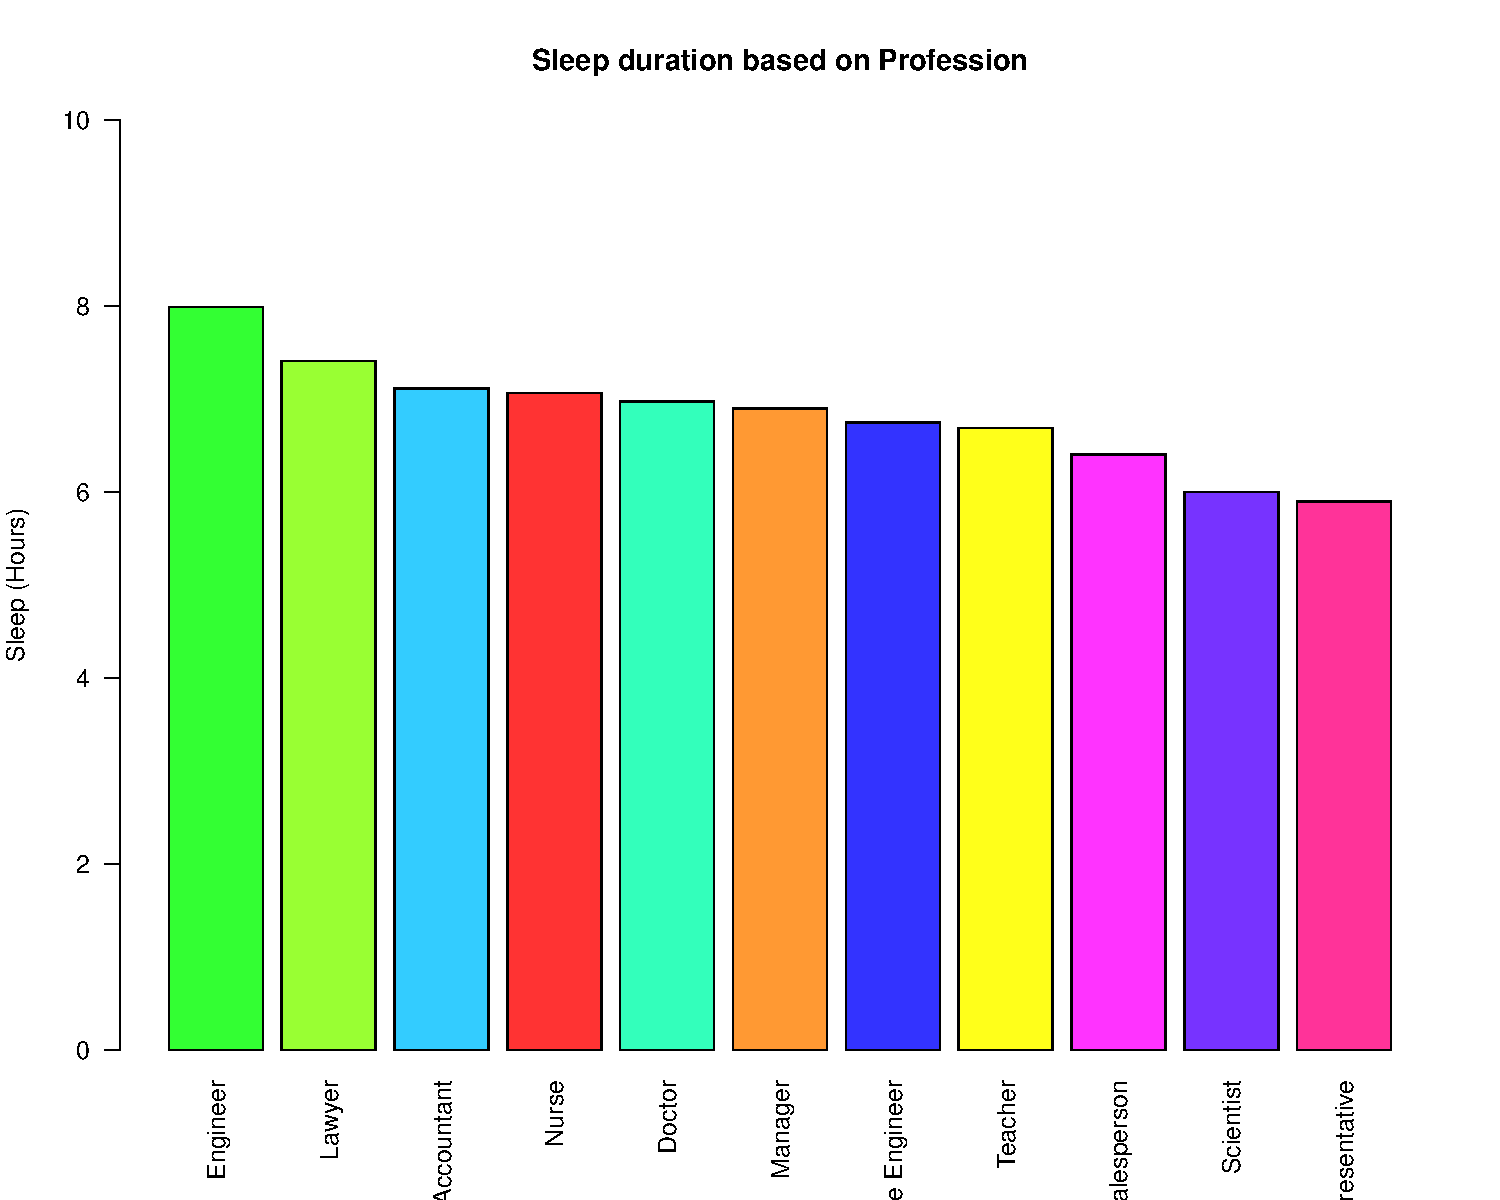
\includegraphics[keepaspectratio]{Sleepcase_files/figure-pdf/unnamed-chunk-4-1.pdf}}

\emph{Engineer is with the highest duration of sleep on average}

\begin{Shaded}
\begin{Highlighting}[]
\NormalTok{sleepocqw}\OtherTok{\textless{}{-}}\FunctionTok{aggregate}\NormalTok{( sleep\_quality }\SpecialCharTok{\textasciitilde{}}\NormalTok{ occupation, }\AttributeTok{data =}\NormalTok{ sleep, }\AttributeTok{FUN =}\NormalTok{ mean)}
\NormalTok{sleepocqw}\OtherTok{\textless{}{-}}\FunctionTok{cbind}\NormalTok{(sleepocqw,coljack)}
\NormalTok{sleepocqw }\OtherTok{\textless{}{-}}\NormalTok{ sleepocqw[}\FunctionTok{order}\NormalTok{(}\SpecialCharTok{{-}}\NormalTok{sleepocqw}\SpecialCharTok{$}\NormalTok{sleep\_quality),]}
\FunctionTok{print}\NormalTok{(sleepocqw)}
\end{Highlighting}
\end{Shaded}

\begin{verbatim}
             occupation sleep_quality coljack
3              Engineer      8.412698 #33ff33
4                Lawyer      7.893617 #99ff33
1            Accountant      7.891892 #33ccff
6                 Nurse      7.369863 #ff3333
5               Manager      7.000000 #ff9933
11              Teacher      6.975000 #ffff1a
2                Doctor      6.647887 #33ffbb
10    Software Engineer      6.500000 #3333ff
8           Salesperson      6.000000 #ff33ff
9             Scientist      5.000000 #7733ff
7  Sales Representative      4.000000 #ff3399
\end{verbatim}

\begin{Shaded}
\begin{Highlighting}[]
\FunctionTok{par}\NormalTok{(}\AttributeTok{mar =} \FunctionTok{c}\NormalTok{(}\DecValTok{10}\NormalTok{, }\DecValTok{4}\NormalTok{, }\DecValTok{4}\NormalTok{, }\DecValTok{2}\NormalTok{))}
\FunctionTok{barplot}\NormalTok{(sleepocqw}\SpecialCharTok{$}\NormalTok{sleep\_quality,}
        \AttributeTok{names.arg =}\NormalTok{ sleepocqw}\SpecialCharTok{$}\NormalTok{occupation,}
        \AttributeTok{col =}\NormalTok{ sleepocqw}\SpecialCharTok{$}\NormalTok{coljack,}
        \AttributeTok{main =} \StringTok{"Sleep quality based on Profession"}\NormalTok{,}
        \AttributeTok{axis.lty =} \DecValTok{0}\NormalTok{,}
        \AttributeTok{las=}\DecValTok{2}\NormalTok{,}
        \AttributeTok{ylim =} \FunctionTok{c}\NormalTok{(}\DecValTok{0}\NormalTok{,}\DecValTok{10}\NormalTok{),}
        \AttributeTok{ylab =} \StringTok{"Sleep quality (1{-}10)"}
        
\NormalTok{        )}
\end{Highlighting}
\end{Shaded}

\pandocbounded{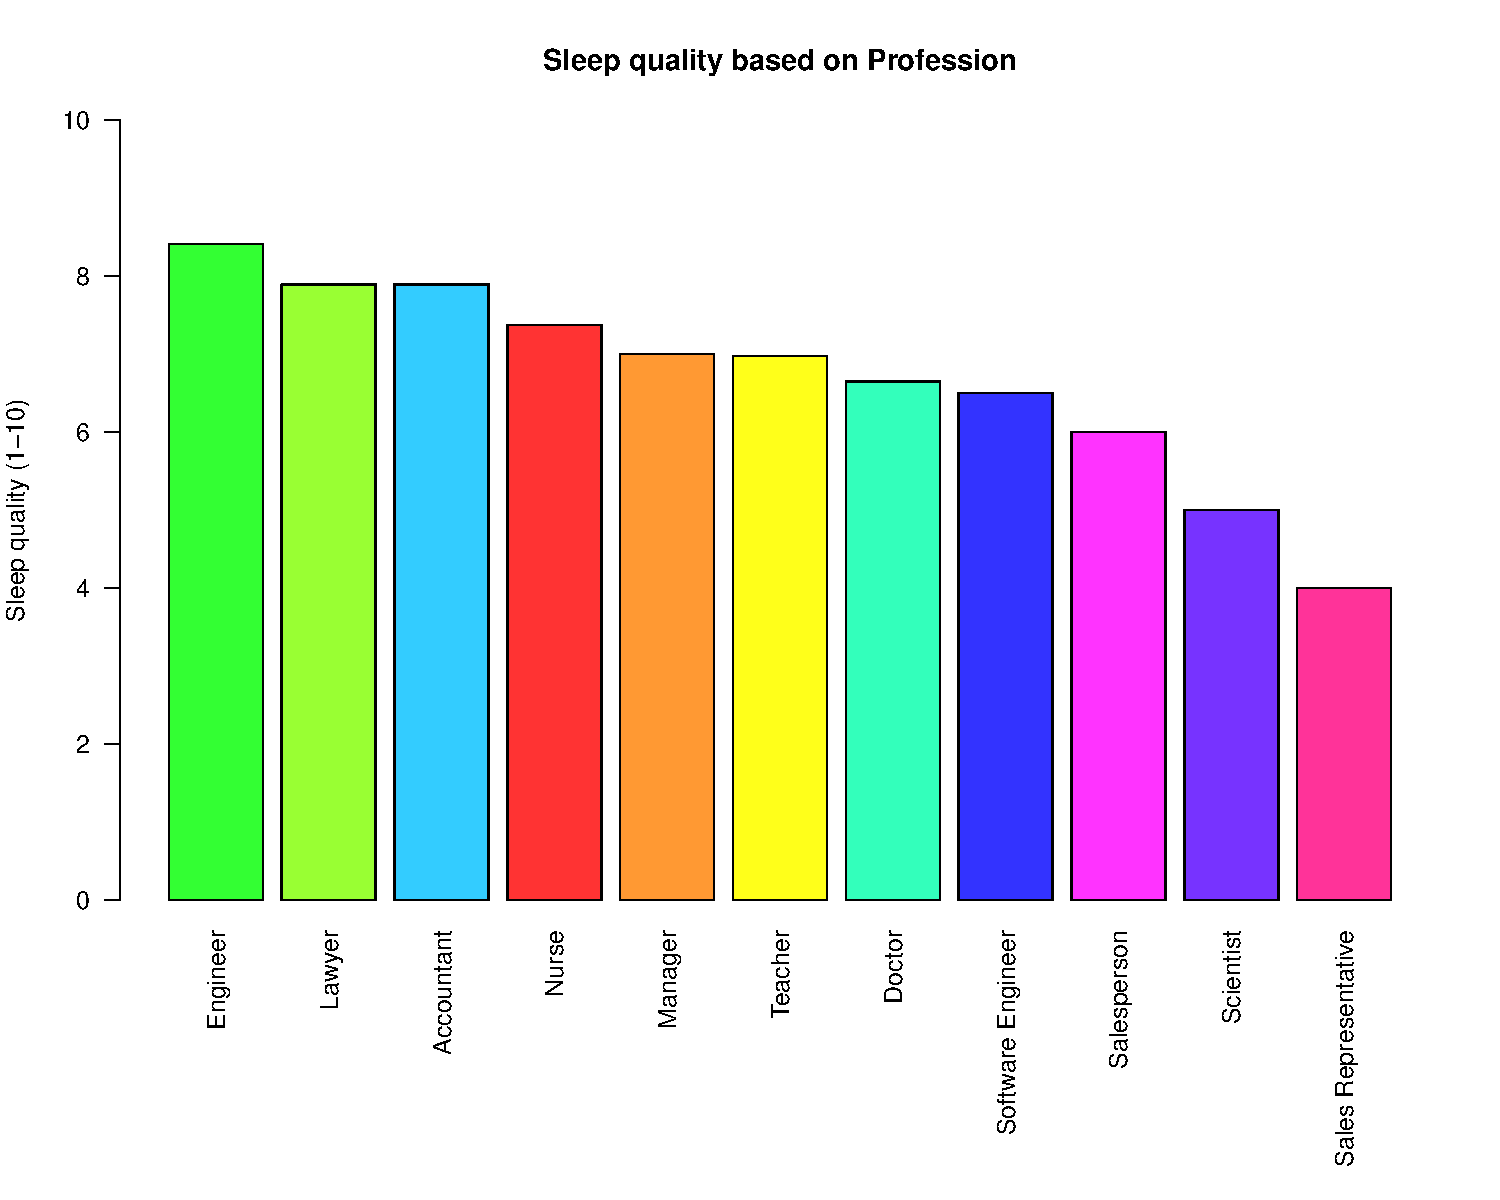
\includegraphics[keepaspectratio]{Sleepcase_files/figure-pdf/unnamed-chunk-5-1.pdf}}

\begin{Shaded}
\begin{Highlighting}[]
\NormalTok{sleepocst}\OtherTok{\textless{}{-}}\FunctionTok{aggregate}\NormalTok{(stress\_level }\SpecialCharTok{\textasciitilde{}}\NormalTok{ occupation, }\AttributeTok{data =}\NormalTok{ sleep, }\AttributeTok{FUN =}\NormalTok{ mean )}
\NormalTok{sleepocst}\OtherTok{\textless{}{-}}\FunctionTok{cbind}\NormalTok{(sleepocst,coljack)}
\NormalTok{sleepocst}\OtherTok{\textless{}{-}}\NormalTok{sleepocst[}\FunctionTok{order}\NormalTok{(}\SpecialCharTok{{-}}\NormalTok{sleepocst}\SpecialCharTok{$}\NormalTok{stress\_level),]}
\FunctionTok{print}\NormalTok{(sleepocst)}
\end{Highlighting}
\end{Shaded}

\begin{verbatim}
             occupation stress_level coljack
7  Sales Representative     8.000000 #ff3399
8           Salesperson     7.000000 #ff33ff
9             Scientist     7.000000 #7733ff
2                Doctor     6.732394 #33ffbb
10    Software Engineer     6.000000 #3333ff
6                 Nurse     5.547945 #ff3333
4                Lawyer     5.063830 #99ff33
5               Manager     5.000000 #ff9933
1            Accountant     4.594595 #33ccff
11              Teacher     4.525000 #ffff1a
3              Engineer     3.888889 #33ff33
\end{verbatim}

\begin{Shaded}
\begin{Highlighting}[]
\NormalTok{bpst}\OtherTok{\textless{}{-}}\FunctionTok{barplot}\NormalTok{(sleepocst}\SpecialCharTok{$}\NormalTok{stress\_level, }\AttributeTok{col =}\NormalTok{ sleepocst}\SpecialCharTok{$}\NormalTok{coljack,  }\AttributeTok{main =} \StringTok{"Occupation and stress level"}\NormalTok{, }\AttributeTok{ylab =} \StringTok{"Stress level (1{-}10)"}\NormalTok{, }\AttributeTok{ylim =} \FunctionTok{c}\NormalTok{(}\DecValTok{0}\NormalTok{,}\DecValTok{10}\NormalTok{), )}

\FunctionTok{text}\NormalTok{(}\AttributeTok{x =}\NormalTok{ bpst, }\AttributeTok{y =}\NormalTok{ sleepocst}\SpecialCharTok{$}\NormalTok{stress\_level }\SpecialCharTok{+} \FloatTok{0.3}\NormalTok{, }\AttributeTok{labels =}\NormalTok{ sleepocst}\SpecialCharTok{$}\NormalTok{occupation, }\AttributeTok{srt =} \DecValTok{90}\NormalTok{,}\AttributeTok{adj =} \DecValTok{0}\NormalTok{,}\AttributeTok{cex =} \DecValTok{1}
\NormalTok{)}
\end{Highlighting}
\end{Shaded}

\pandocbounded{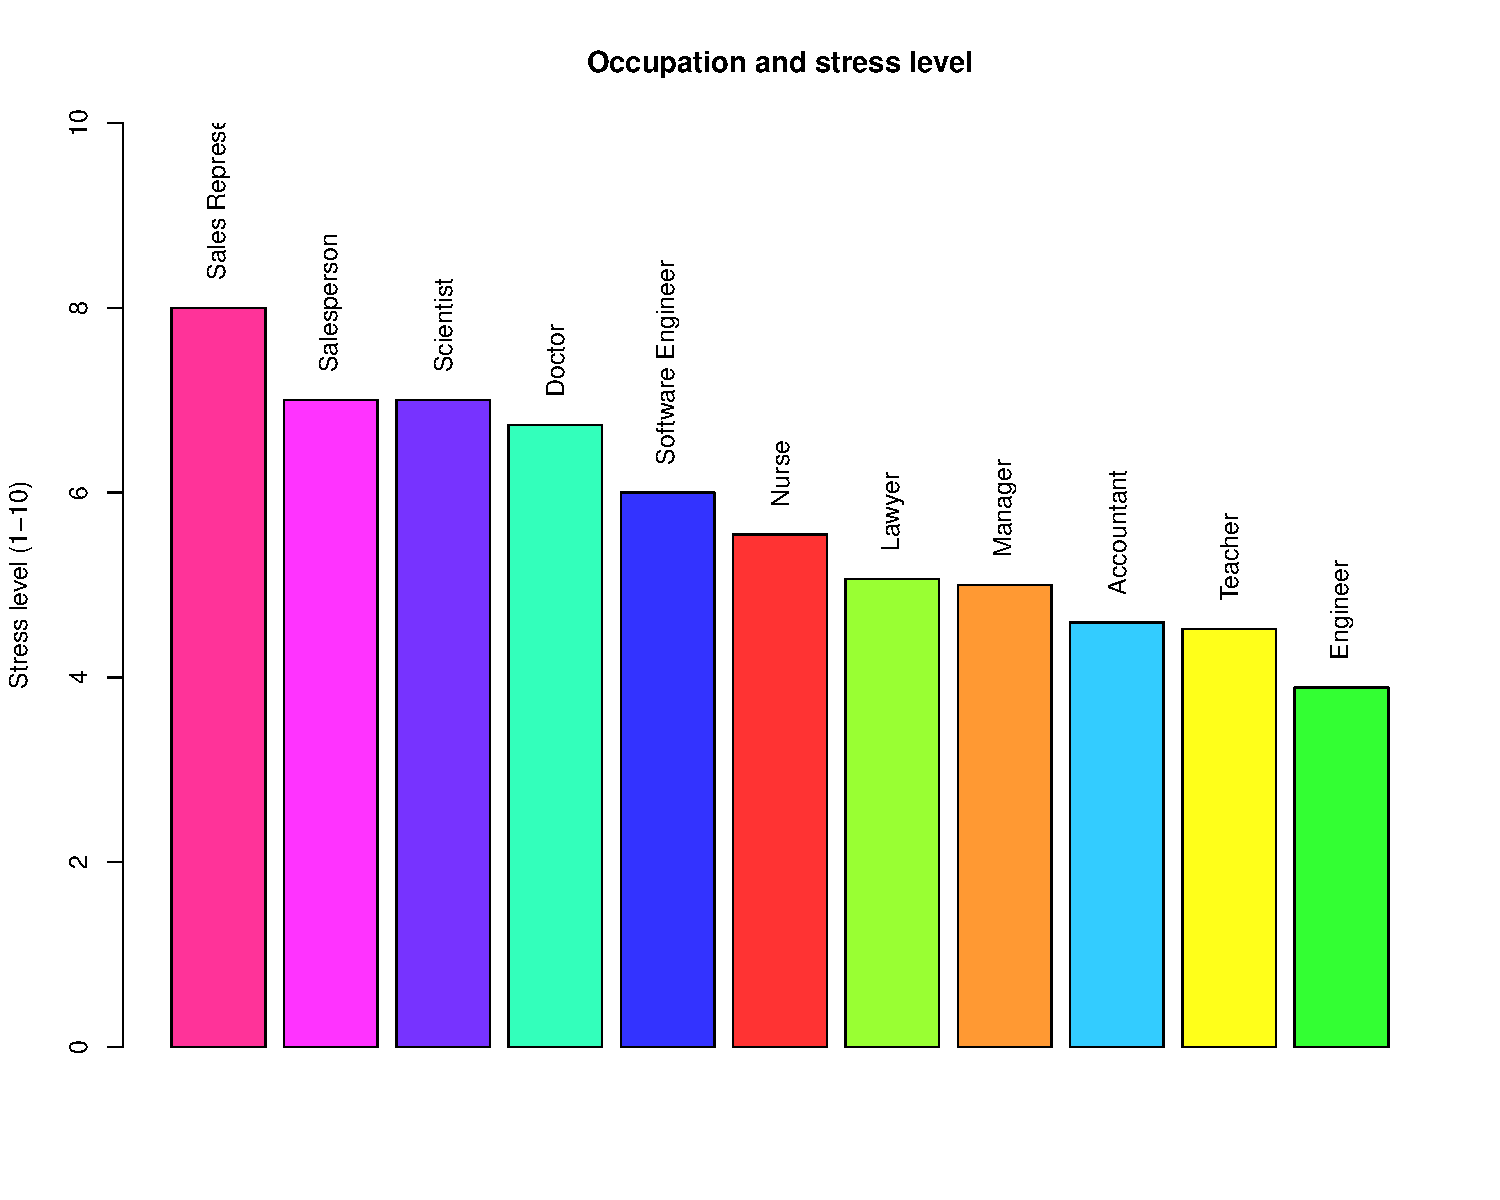
\includegraphics[keepaspectratio]{Sleepcase_files/figure-pdf/unnamed-chunk-6-1.pdf}}

\textbf{\emph{Sleep disorder}}

\begin{Shaded}
\begin{Highlighting}[]
\FunctionTok{table}\NormalTok{(sleep}\SpecialCharTok{$}\NormalTok{sleep\_disorder)}
\end{Highlighting}
\end{Shaded}

\begin{verbatim}

   Insomnia        None Sleep Apnea 
         77         219          78 
\end{verbatim}

Sleep Apnea is most common (excluding no disorder)

\begin{Shaded}
\begin{Highlighting}[]
\NormalTok{sleep\_male}\OtherTok{\textless{}{-}}\NormalTok{sleep[sleep}\SpecialCharTok{$}\NormalTok{gender }\SpecialCharTok{\%in\%} \FunctionTok{c}\NormalTok{(}\StringTok{"Male"}\NormalTok{),]}
\CommentTok{\#Male}
\FunctionTok{table}\NormalTok{(sleep\_male}\SpecialCharTok{$}\NormalTok{sleep\_disorder)}
\end{Highlighting}
\end{Shaded}

\begin{verbatim}

   Insomnia        None Sleep Apnea 
         41         137          11 
\end{verbatim}

\begin{Shaded}
\begin{Highlighting}[]
\NormalTok{sleep\_female}\OtherTok{\textless{}{-}}\NormalTok{sleep[sleep}\SpecialCharTok{$}\NormalTok{gender }\SpecialCharTok{\%in\%} \FunctionTok{c}\NormalTok{(}\StringTok{"Female"}\NormalTok{),]}
\CommentTok{\#Female}
\FunctionTok{table}\NormalTok{(sleep\_female}\SpecialCharTok{$}\NormalTok{sleep\_disorder)}
\end{Highlighting}
\end{Shaded}

\begin{verbatim}

   Insomnia        None Sleep Apnea 
         36          82          67 
\end{verbatim}

Most common in Male is Insomnia Most common in Female is Apnea

\begin{Shaded}
\begin{Highlighting}[]
\NormalTok{sleepocst\_Male}\OtherTok{\textless{}{-}}\FunctionTok{aggregate}\NormalTok{(stress\_level }\SpecialCharTok{\textasciitilde{}}\NormalTok{ occupation, }\AttributeTok{data =}\NormalTok{ sleep\_male, }\AttributeTok{FUN =}\NormalTok{ mean )}
\NormalTok{sleepocst\_Male}\OtherTok{\textless{}{-}}\NormalTok{sleepocst\_Male[}\FunctionTok{order}\NormalTok{(}\SpecialCharTok{{-}}\NormalTok{sleepocst\_Male}\SpecialCharTok{$}\NormalTok{stress\_level),]}
\FunctionTok{print}\NormalTok{(sleepocst\_Male)}
\end{Highlighting}
\end{Shaded}

\begin{verbatim}
            occupation stress_level
5 Sales Representative     8.000000
6          Salesperson     7.000000
2               Doctor     6.840580
8              Teacher     6.200000
1           Accountant     6.000000
7    Software Engineer     6.000000
4               Lawyer     5.044444
3             Engineer     4.806452
\end{verbatim}

Male Sales Representatives has highest stress

\begin{Shaded}
\begin{Highlighting}[]
\NormalTok{sleepocst\_Female}\OtherTok{\textless{}{-}}\FunctionTok{aggregate}\NormalTok{(stress\_level }\SpecialCharTok{\textasciitilde{}}\NormalTok{ occupation, }\AttributeTok{data =}\NormalTok{ sleep\_female, }\AttributeTok{FUN =}\NormalTok{ mean )}
\NormalTok{sleepocst\_Female}\OtherTok{\textless{}{-}}\NormalTok{sleepocst\_Female[}\FunctionTok{order}\NormalTok{(}\SpecialCharTok{{-}}\NormalTok{sleepocst\_Female}\SpecialCharTok{$}\NormalTok{stress\_level),]}
\FunctionTok{print}\NormalTok{(sleepocst\_Female)}
\end{Highlighting}
\end{Shaded}

\begin{verbatim}
  occupation stress_level
7  Scientist     7.000000
6      Nurse     5.547945
4     Lawyer     5.500000
5    Manager     5.000000
1 Accountant     4.555556
8    Teacher     4.285714
2     Doctor     3.000000
3   Engineer     3.000000
\end{verbatim}

Female Scientist has highest stress

\begin{Shaded}
\begin{Highlighting}[]
\NormalTok{sleepocqw\_male}\OtherTok{\textless{}{-}}\FunctionTok{aggregate}\NormalTok{( sleep\_quality }\SpecialCharTok{\textasciitilde{}}\NormalTok{ occupation, }\AttributeTok{data =}\NormalTok{ sleep\_male, }\AttributeTok{FUN =}\NormalTok{ mean)}
\NormalTok{sleepocqw\_male }\OtherTok{\textless{}{-}}\NormalTok{ sleepocqw\_male[}\FunctionTok{order}\NormalTok{(}\SpecialCharTok{{-}}\NormalTok{sleepocqw\_male}\SpecialCharTok{$}\NormalTok{sleep\_quality),]}
\FunctionTok{print}\NormalTok{(sleepocqw\_male)}
\end{Highlighting}
\end{Shaded}

\begin{verbatim}
            occupation sleep_quality
1           Accountant      8.000000
4               Lawyer      7.933333
3             Engineer      7.806452
2               Doctor      6.579710
7    Software Engineer      6.500000
6          Salesperson      6.000000
8              Teacher      6.000000
5 Sales Representative      4.000000
\end{verbatim}

Lowsest Male sleep quality is for Sales Representatives

\begin{Shaded}
\begin{Highlighting}[]
\NormalTok{sleepocqw\_female}\OtherTok{\textless{}{-}}\FunctionTok{aggregate}\NormalTok{( sleep\_quality }\SpecialCharTok{\textasciitilde{}}\NormalTok{ occupation, }\AttributeTok{data =}\NormalTok{ sleep\_female, }\AttributeTok{FUN =}\NormalTok{ mean)}
\NormalTok{sleepocqw\_female }\OtherTok{\textless{}{-}}\NormalTok{ sleepocqw\_female[}\FunctionTok{order}\NormalTok{(}\SpecialCharTok{{-}}\NormalTok{sleepocqw\_female}\SpecialCharTok{$}\NormalTok{sleep\_quality),]}
\FunctionTok{print}\NormalTok{(sleepocqw\_female)}
\end{Highlighting}
\end{Shaded}

\begin{verbatim}
  occupation sleep_quality
2     Doctor      9.000000
3   Engineer      9.000000
1 Accountant      7.888889
6      Nurse      7.369863
8    Teacher      7.114286
4     Lawyer      7.000000
5    Manager      7.000000
7  Scientist      5.000000
\end{verbatim}

Lowest Female sleep quality is for Scientist

\begin{Shaded}
\begin{Highlighting}[]
\FunctionTok{print}\NormalTok{(}\FunctionTok{cor}\NormalTok{(sleep}\SpecialCharTok{$}\NormalTok{sleep\_quality,sleep}\SpecialCharTok{$}\NormalTok{stress\_level))}
\end{Highlighting}
\end{Shaded}

\begin{verbatim}
[1] -0.898752
\end{verbatim}

There is a negative correlation between stress level and sleep quality
meaning the more stress a person have the worse is there sleep quality.
Also basing that there is a similar correlation in separate female and
male group i think that there is enough evidence to say there can be a
strong correlation.

\begin{Shaded}
\begin{Highlighting}[]
\NormalTok{ sleep\_male\_insomnia}\OtherTok{\textless{}{-}}\NormalTok{sleep\_male[sleep\_male}\SpecialCharTok{$}\NormalTok{sleep\_disorder }\SpecialCharTok{\%in\%} \FunctionTok{c}\NormalTok{(}\StringTok{"Insomnia"}\NormalTok{),]}
\FunctionTok{print}\NormalTok{(}\FunctionTok{length}\NormalTok{(sleep\_male\_insomnia}\SpecialCharTok{$}\NormalTok{gender)}\SpecialCharTok{/}\FunctionTok{length}\NormalTok{(sleep\_male}\SpecialCharTok{$}\NormalTok{gender)}\SpecialCharTok{*}\DecValTok{100}\NormalTok{)}
\end{Highlighting}
\end{Shaded}

\begin{verbatim}
[1] 21.69312
\end{verbatim}

Wrong 21.69 percent of males strugle from Insomnoa

\begin{Shaded}
\begin{Highlighting}[]
\FunctionTok{print}\NormalTok{(}\FunctionTok{mean}\NormalTok{(sleep\_male\_insomnia}\SpecialCharTok{$}\NormalTok{daily\_steps))}
\end{Highlighting}
\end{Shaded}

\begin{verbatim}
[1] 5812.195
\end{verbatim}

Wring the average daily steps by males with insomnia is 5812

\begin{Shaded}
\begin{Highlighting}[]
\NormalTok{sleep\_insomnia}\OtherTok{\textless{}{-}}\NormalTok{sleep[sleep}\SpecialCharTok{$}\NormalTok{sleep\_disorder }\SpecialCharTok{\%in\%} \FunctionTok{c}\NormalTok{(}\StringTok{"Insomnia"}\NormalTok{),]}
\FunctionTok{summary}\NormalTok{(sleep\_insomnia}\SpecialCharTok{$}\NormalTok{sleep\_duration)}
\end{Highlighting}
\end{Shaded}

\begin{verbatim}
   Min. 1st Qu.  Median    Mean 3rd Qu.    Max. 
   5.90    6.40    6.50    6.59    6.60    8.30 
\end{verbatim}

\begin{Shaded}
\begin{Highlighting}[]
\FunctionTok{boxplot}\NormalTok{(sleep\_insomnia}\SpecialCharTok{$}\NormalTok{sleep\_duration, }\AttributeTok{horizontal =} \ConstantTok{TRUE}\NormalTok{, }\AttributeTok{main =} \StringTok{"Duration of sleep with Insomnia"}\NormalTok{)}
\end{Highlighting}
\end{Shaded}

\pandocbounded{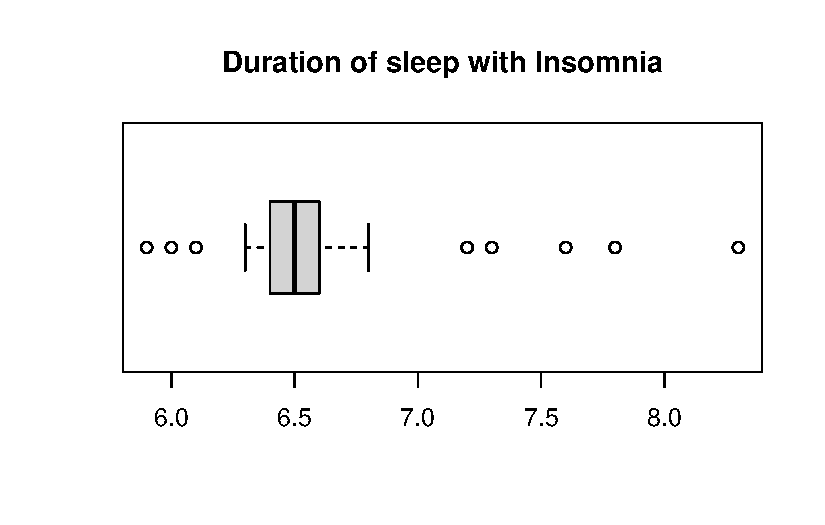
\includegraphics[keepaspectratio]{Sleepcase_files/figure-pdf/unnamed-chunk-15-1.pdf}}

\begin{Shaded}
\begin{Highlighting}[]
\NormalTok{sleep\_apnea}\OtherTok{\textless{}{-}}\NormalTok{sleep[sleep}\SpecialCharTok{$}\NormalTok{sleep\_disorder }\SpecialCharTok{\%in\%} \FunctionTok{c}\NormalTok{(}\StringTok{"Sleep Apnea"}\NormalTok{),]}
\FunctionTok{print}\NormalTok{(}\FunctionTok{summary}\NormalTok{(sleep\_apnea}\SpecialCharTok{$}\NormalTok{sleep\_duration))}
\end{Highlighting}
\end{Shaded}

\begin{verbatim}
   Min. 1st Qu.  Median    Mean 3rd Qu.    Max. 
  5.800   6.100   6.800   7.032   8.100   8.200 
\end{verbatim}

\begin{Shaded}
\begin{Highlighting}[]
\FunctionTok{boxplot}\NormalTok{(sleep\_apnea}\SpecialCharTok{$}\NormalTok{sleep\_duration, }\AttributeTok{horizontal =} \ConstantTok{TRUE}\NormalTok{,}\AttributeTok{main =} \StringTok{"Duration of sleep with Sleep Apnea"}\NormalTok{)}
\end{Highlighting}
\end{Shaded}

\pandocbounded{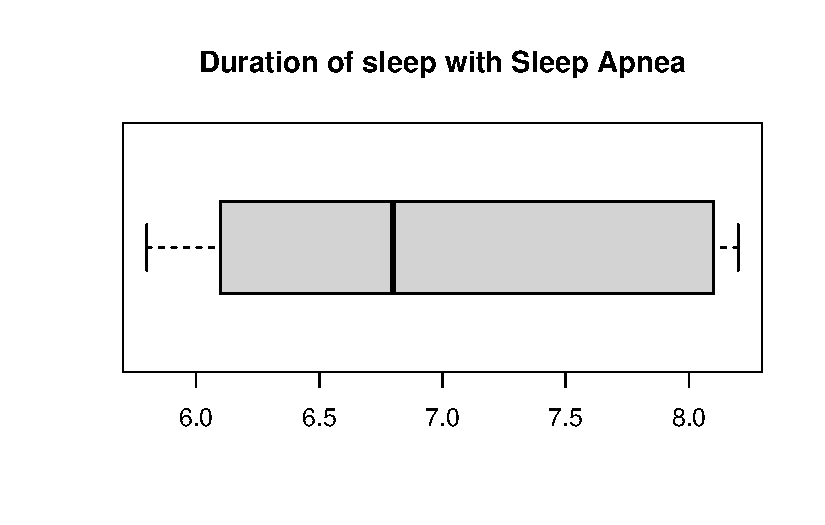
\includegraphics[keepaspectratio]{Sleepcase_files/figure-pdf/unnamed-chunk-15-2.pdf}}




\end{document}
